\section{Participation notes 9}
Participant: Student

\begin{itemize}
    \item \textbf{Have them read the code-example} - The user mentions being confused by the task.
    \item \textbf{Have them draw the structure} - The participant explains drawing the namespace as a separate thing with two functions in it. The two functions print and are called by main which is outside the namespace.
    \item \textbf{Have them submit the git URL} - User writes into the git repository field and reads the description before clicking the submit button. The participant then mentions seeing a line before navigating using the mouse. 
    \item \textbf{Have them get the main() implementation} - The user clicks the main function and says it is possible to view the implementation, but seem confused when trying to get the other functions. First saying it is not possible before changing opinion. 
    \item \textbf{Participant visualization} \includepdf[pages={9}]{inc/generalAppendix/userStudies/participantsVisualization.pdf}
\end{itemize}